\documentclass[11pt, oneside]{article} 
\usepackage{geometry}
\geometry{letterpaper} 
\usepackage{graphicx}
	
\usepackage{amssymb}
\usepackage{amsmath}
\usepackage{parskip}
\usepackage{color}
\usepackage{hyperref}

\graphicspath{{/Users/telliott/Github/calculus_book/png/}}
% \begin{center} 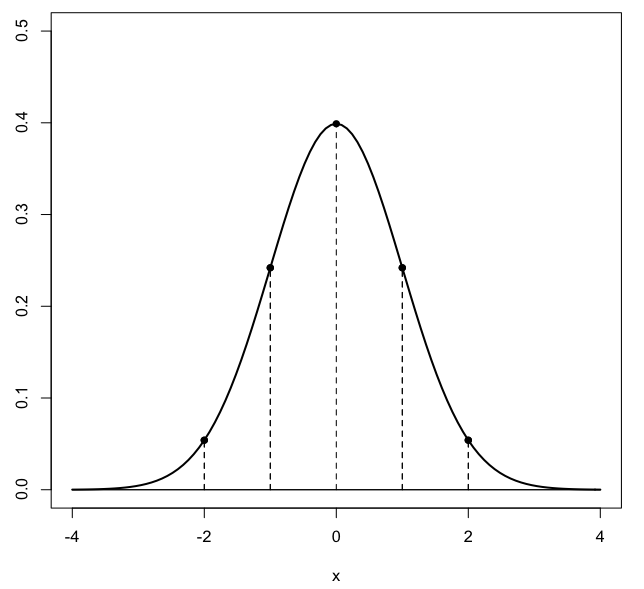
\includegraphics [scale=0.4] {gauss3.png} \end{center}

\title{Euclid's Elements}
\date{}

\begin{document}
\maketitle
\Large

In this chapter we look at the first few \emph{Propositions} in Euclid's \emph{Elements}, meant to be a textbook of geometry for students.  We will see how the propositions build on one another.  

The first three are \emph{constructions}, e.g. the very first is the construction of a triangle with all three sides equal, an equilateral triangle.

\subsection*{Prop. I.1}
To construct an equilateral triangle on a given line segment.
\begin{center} 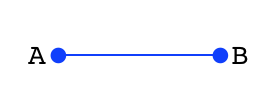
\includegraphics [scale=0.4] {PI_1a.png} \end{center}

The tools we have are a straightedge and a compass.  The compass is collapsible, meaning that it cannot be used to transfer distances since it loses its setting when lifted from the page.  As we'll see in the next part, this is a problem that can be solved.

Euclid was smart enough to know about compasses and how to set them.  The idea is:  to have the fewest possible assumptions, and a non-collapsible compass was a luxury he didn't need, since he could accomplish the same end without it, as we will see.

The first step is to draw two circles on centers $A$ and $B$.
\begin{center} 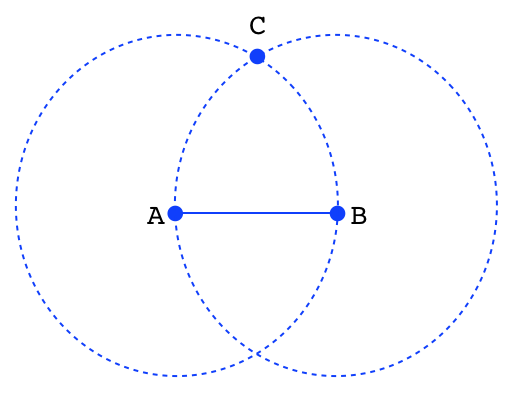
\includegraphics [scale=0.4] {PI_1b.png} \end{center}

The circles are drawn with each radius equal to the line segment $AB$.  It is a property of circles that all points on the circle are at the same distance from the center.  Thus all points on the left-hand circle are equidistant from $A$, and all points on the second one are equidistant from $B$.  

Therefore, the point $C$  where the circles cross is equidistant from \emph{both} $A$ and $B$ (there is another at the bottom).

We don't really need the entire circle, just the part where the arcs cross at $C$.

\begin{center} 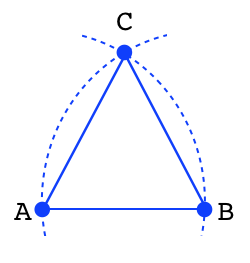
\includegraphics [scale=0.4] {PI_1c.png} \end{center}

Use the straight edge to draw $\triangle ABC$.  Since $AC = AB$ and $BC = AB$, we know that $AC = BC$.  The triangle is equilateral.

The proof doesn't stand on its own.  We used a definition (D) and a common notion (CN).

$\circ$ \ D I.15  all radii of a circle are equal.

$\circ$ \ CN I.1  things which equal the same thing also equal one another.

We put a little box to show that the proof is complete.

$\square$

\subsection*{Prop. I.2}
To place a straight line equal to a given straight line with one end at a given point.

We will construct a line segment at $A$ equal in length to $BC$ (left panel).  The first thing is to draw the line segment $AB$ and construct an equilateral triangle on it (right panel).   
\begin{center} 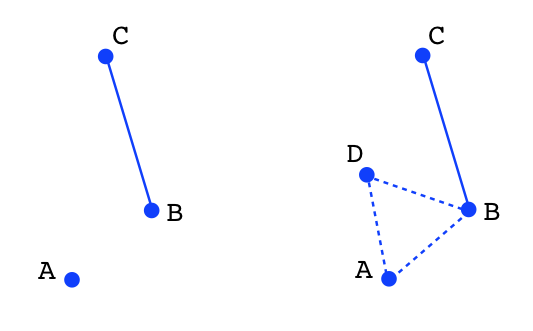
\includegraphics [scale=0.4] {PI_2a.png} \end{center}

We know how to do this ($P I.1$).  

Next, construct a circle on center $B$ with radius $BC$ and extend the line segment $DB$ to point $G$.  Now construct a circle on center $D$ with radius $DG$ and extend $DA$ to that circle at point $L$.  

We have:

\begin{center} 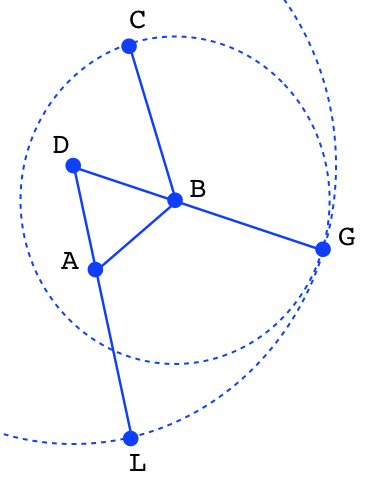
\includegraphics [scale=0.4] {PI_2b.png} \end{center}

As common radii of the circle on center $B$, we have $BC = BG$.  

As common radii of the circle on center $D$, we have $DL = DG$.  

As sides of an equilateral triangle, we have $DA = DB$.

We use CN I.3:  if equals are subtracted from equals, then the remainders are equal.  Thus, $AL = BG$.  But we had above that $BC = BG$.  Therefore, $AL = BC$, by CN I.1.  

Q.E.D. or "quod erat demonstrandum", which is Latin, and in the original Greek \emph{the very thing it was required to have shown.}. 

$\square$

Note in passing, the orientation is given by $AB$.  We have not shown how to transfer the length with an arbitrary orientation.  We will solve this next.

\subsection*{Prop. I.3}
To cut off the lesser of two unequal straight lines from the greater.

\begin{center} 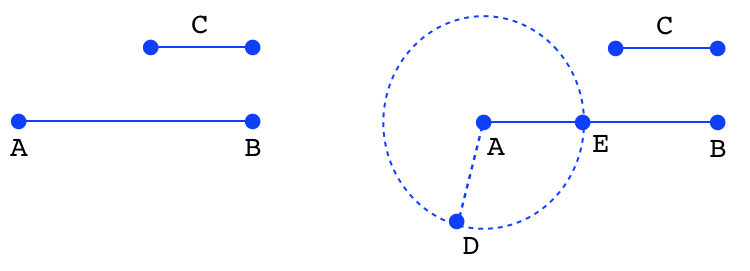
\includegraphics [scale=0.4] {PI_3a.png} \end{center}

In the left panel, we have the line segment $AB$ and a smaller one just labeled $C$.  To do the construction, use the method of $P I.2$ and transfer $C$ to point $A$, forming $AD$.  

Next, use $AD$ as the radius of a circle on center $A$.  Then, $AE = AD$, but $AD = C$.  Hence $BE = AB - C$, as required.

$\square$

At this point, we have a method to mark off a given length on a larger length, even though all we have is a collapsing compass.  Therefore, going forward, we can act as if we have a standard compass, that holds its setting after being lifted from the paper.

We also have the means to an important \emph{trichotomy}.  Comparing two line segments, one of three things is true:  the first is smaller than the second, they are equal, or the second is smaller than the first.

\subsection*{Prop. I.4}

\begin{quote}If two triangles have two sides equal to two sides respectively, and have the angles contained by the equal straight lines equal, then they also have the base equal to the base, the triangle equals the triangle, and the remaining angles equal the remaining angles respectively, namely those opposite the equal sides.\end{quote}

\begin{center} 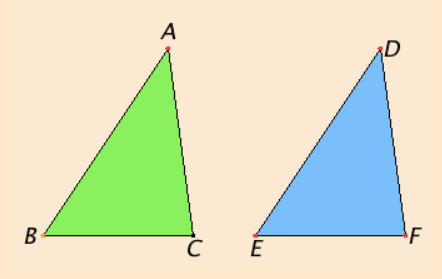
\includegraphics [scale=0.4] {PI_4a.png} \end{center}

This is not a construction, unlike the previous three propositions.  It is a method for proving congruence (equality) of two triangles 
\[ \triangle ABC \cong \triangle DEF \]

Elsewhere in this book we would call the method SAS or \emph{side angle side}.  Given that $AB = DE$ and $AC = DF$ and that the angles between them at the vertices $A$ and $D$ are also equal, the two triangles are congruent:  all three and angles and all three sides are equal.

This is a proof that SAS is correct.

The proof is by superposition.  The facts establish the positions of the points $B$ and $C$.  Euclid says that if we lift up $\triangle ABC$ and lay it on top of $\triangle DEF$ then $B$ coincides with $E$ and $C$ coincides with $F$ so $BC = EF$.

This seems perhaps a little shaky logically, it's not a method of proof that Euclid likes.

But one might instead have taken this proposition as a postulate.  The source, above, says that David Hilbert claims that under the hypotheses of the proposition it is true that the two base angles are equal, and then proves that the bases are equal.

We have used SAS to prove SSS, that all three sides are equal.

In any event, SAS is very commonly used to prove congruence.  
\begin{center} 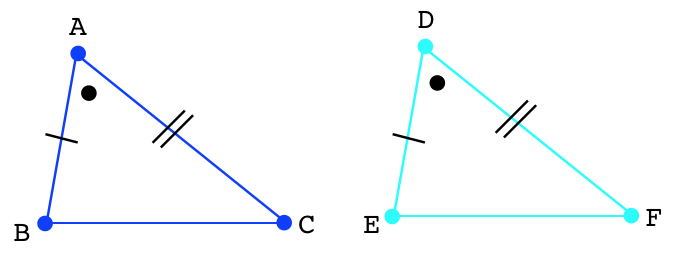
\includegraphics [scale=0.4] {PI_4b.png} \end{center}

In this diagram, sides of equal length are indicated by one or more hash marks.  Equal angles are indicated by dots (another common method is to draw an arc with a hash across it).

The other methods for proving congruence use two equal angles and a side.  Two equal angles imply the third angle is also equal (since they add to a half-circle or 180 degrees), so the two triangles are similar.  To prove they are congruent, It is important that the equal sides are flanked by the same angles, or equivalently, are opposite the same angle.

These methods using two angles are referred to as ASA and AAS.

The next proposition refers to triangles with just two equal sides, called isosceles.

\subsection*{Prop. I.5}

\begin{quote}In isosceles triangles the angles at the base equal one another, and, if the equal straight lines are produced further, then the angles under the base equal one another.\end{quote}

\begin{center} 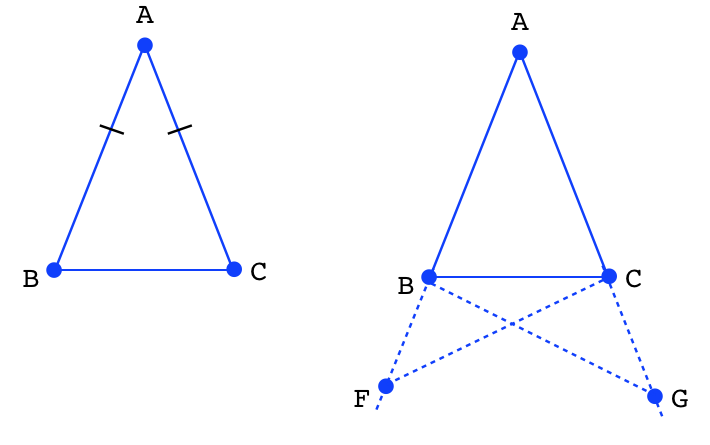
\includegraphics [scale=0.3] {PI_5a.png} \end{center}

We are given that $AB = AC$.  Extend the sides downward to $D$ and $E$ (not shown) and mark off equal distances $AF = AG$.

$\circ$ \ (0) given that $AB = AC$ and $AF = AG$

$\circ$ \ (1) $\triangle ACF \cong \triangle ABG$ [by SAS]

\begin{center} 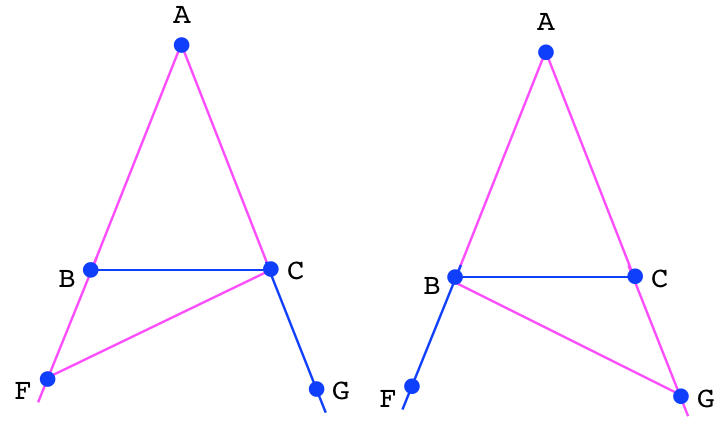
\includegraphics [scale=0.3] {PI_5b.png} \end{center}

$\circ$ \ (2) $\angle ACF = \angle ABG$ and $FC = BG$ [by congruent $\triangle$ from (1)]

$\circ$ \ (3) Further, $BF = CB$ [by subtraction, using (0)].

$\circ$ \ (4) $\triangle BCF \cong BCG$ by SSS.

\begin{center} 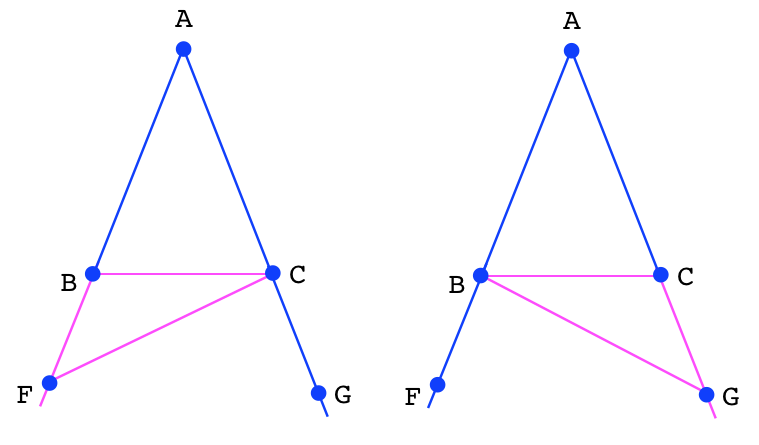
\includegraphics [scale=0.3] {PI_5c.png} \end{center}

$\circ$ \ (5) $\angle FBC = \angle BCG$ by congruent $\triangle$ in (4).

At this point we would use supplementary angles to finish the proof, but Euclid does not allow himself to do that.

$\circ$ \ (5) $\angle BCF = \angle CBG$ by congruent $\triangle$ from (4)

$\circ$ \ (7) $\angle ABG - \angle CBG = \angle ABC$.

$\circ$ \ (8) $\angle ACF - \angle BCF = \angle ACB$.

$\circ$ \ (9) But $\angle ABG = \angle ACF$ (2) and $\angle BCF = \angle CBG$ (5), so by subtraction we obtain equals and therefore have
\[ \angle ABC = \angle ACB \]

$\square$

We will prove the converse \hyperref[sec:isosceles_backward]{\textbf{here}}.

Euclid's proof of the converse is shorter and introduces the method of contradiction, or \emph{reductio ad absurdum}.  That is the next proposition.
  
\subsection*{Prop. I.6}

If in a triangle two angles equal one another, then the sides opposite the equal angles also equal one another.

Suppose we have $\triangle ABC$ with $\angle ABC = \angle ACB$.

\begin{center} 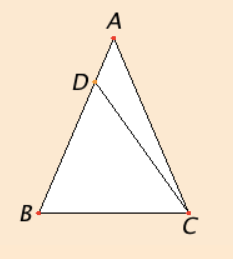
\includegraphics [scale=0.5] {PI_6a.png} \end{center}

If $AB$ does not equal $AC$, then one of them is greater.  Let $AB$ be greater, then cut off $DB$ from $AB$ such that $DB = AC$.

\begin{quote}Since $DB$ equals $AC$, and $BC$ is common, therefore the two sides $DB$ and $BC$ equal the two sides $AC$ and $CB$ respectively, and the $\angle DBC$ equals $\angle ACB$. 

Therefore the base $DC$ equals the base $AB$, and $\triangle DBC$ equals $\triangle ACB$, the less equals the greater, which is absurd. Therefore $AB$ cannot be unequal to $AC$, 

It therefore equals it.\end{quote}

In other words, we use SAS to prove that triangle $\triangle ABC \cong \triangle DBC$.  But that is absurd, since the whole is greater than the part, $\triangle ABC$ cannot be equal to a part of itself.

Our original assumption that $AB$ does not equal $AC$ must be false.

The Elements is wonderful, but challenging.  I think this is enough to give us a good taste of the basics of Greek geometry of lines and triangles, and methods of proof.  There is more:  Pythagoras, and circles.

\end{document}